% Version 0; preprint format; Written by SH

\documentclass[preprint]{aastex}
\usepackage{emulateapj5}
\usepackage{apjfonts}
\usepackage{amssymb, amsmath}
\usepackage{graphicx}
\usepackage{CJK}
\DeclareGraphicsExtensions{.pdf,.png,.jpg}
\bibliographystyle{apj}

\input psfig.tex

%%%%%%%%%%%%: User Defined Commands %%%%%%%%%%%%

\newdimen\digitwidth    % These five lines change the meaning of
\setbox1=\hbox{0}       % " in the same way, so that it leaves as
\digitwidth=\wd1        % much space as a digit. (Note: All digits
\catcode`"=\active      % are the same width).

% Luis's Definitions
\def\arcsec{{\prime\prime}}
\def\arcmin{{\prime}}
\def\degree{{\circ}}
\def"{\kern\digitwidth}
\def\h{\hskip -3 mm}
\def\aa{{A\&A}}
\def\aas{{ A\&AS}}
\def\aj{{AJ}}
\def\al{$\alpha$}
\def\bet{$\beta$}
\def\amin{$^\prime$}
\def\annrev{{ARA\&A}}
\def\apj{{ApJ}}
\def\apjs{{ApJS}}
\def\asec{$^{\prime\prime}$}
\def\deg{$^{\circ}$}
\def\ddeg{{\rlap.}$^{\circ}$}
\def\dsec{{\rlap.}$^{\prime\prime}$}
\def\cc{cm$^{-3}$}
\def\etal{{\ et al.~}}
\def\flamb{erg s$^{-1}$ cm$^{-2}$ \AA$^{-1}$}
\def\flux{erg s$^{-1}$ cm$^{-2}$}
\def\fnu{erg s$^{-1}$ cm$^{-2}$ Hz$^{-1}$}
\def\hst{{\it HST}}
\def\kms{km s$^{-1}$}
\def\lamb{$\lambda$}
\def\lax{{$\mathrel{\hbox{\rlap{\hbox{\lower4pt\hbox{$\sim$}}}\hbox{$<$}}}$}}
\def\gax{{$\mathrel{\hbox{\rlap{\hbox{\lower4pt\hbox{$\sim$}}}\hbox{$>$}}}$}}
\def\simlt{\lower.5ex\hbox{$\; \buildrel < \over \sim \;$}}
\def\simgt{\lower.5ex\hbox{$\; \buildrel > \over \sim \;$}}
\def\micron{{$\mu$m}}
\def\mnras{{MNRAS}}
\def\nat{{Nature}}
\def\pasp{{PASP}}
\def\perang{\AA$^{-1}$}
\def\peryr{yr$^{-1}$}
\def\pp{\parshape 2 0truein 6.1truein .3truein 5.5truein}
\def\reference{\noindent\pp}
\def\refindent{\par\noindent\parskip=2pt\hangindent=3pc\hangafter=1 }
\def\sb{mag~arcsec$^{-2}$}
\def\solum{$L_\odot$}
\def\solmass{$M_\odot$}
\def\sigs{$\sigma_*$}
\newcommand{\lt}{<}
\newcommand{\gt}{>}

%Song Huang's definition 
\def\galfit{{\tt GALFIT}}
\def\ser{{S\'{e}rsic\ }}

%%%%%%%%%%%%: Header and Version %%%%%%%%%%%%

\slugcomment{Draft version 0}
\shorttitle{ENVIRONMENT DEPENDENCE OF MASS-SIZE RELATION}
\shortauthors{HUANG ET AL.}

\begin{document}

\begin{CJK*}{UTF8}{gbsn}

%%%%%%%%%%%%: Title and Affiliations %%%%%%%%%%%%

\title{The Environmental Dependence of Structures for Massive Galaxies
from the Hyper-Suprime Camera Survey}

\author{Song Huang (黄崧)\altaffilmark{1} Alexie Leauthaud\altaffilmark{1}, 
Kevin Bundy\altaffilmark{1}, and You}
\date{}                                          

\altaffiltext{1}{Kavli Institute for the Physics and Mathematics of the
Universe, Todai Institutes for Advanced Study, the University of Tokyo (Kavli
IPMU, WPI), Kashiwa 277-8583, Japan}

%%%%%%%%%%%%: Abstract and Keywords %%%%%%%%%%%%

\begin{abstract}

  Many recent observations and numerical simulations suggest that nearby
  massive, early-type galaxies are formed through a ``two-phase'' process.  In
  the proposed second phase, the extended stellar envelope was accumulated
  through many dry mergers. (XX TODO)

\end{abstract}
\keywords{galaxies: elliptical and lenticular, cD --- galaxies: formation --- 
          galaxies: photometry --- galaxies: structure --- galaxies: surveys}

\maketitle

%%%%%%%%%%%%: Main Text %%%%%%%%%%%%

\section{Introduction}

\section{Sample and Data Reduction}

\section{Results}

\section{Discussion}

\section{Summary}

%%%%%%%%%%: Acknowledge %%%%%%%%%%
  
\acknowledgements 
  
  1. Acknowledgements for HSC 
  2. Acknowledgements for Kevin and Alexie's funding 
  3. Acknowledgements for the Python libraries
   
  Funding for SDSS-III has been provided by the Alfred P. Sloan Foundation, the
  Participating Institutions, the National Science Foundation, and the U.S.
  Department of Energy. The SDSS-III web site is http://www.sdss3.org.  SDSS-III
  is managed by the Astrophysical Research Consortium for the Participating
  Institutions of the SDSS-III Collaboration including the University of
  Arizona, the Brazilian Participation Group, Brookhaven National Laboratory,
  University of Cambridge, University of Florida, the French Participation
  Group, the German Participation Group, the Instituto de Astrofisica de
  Canarias, the Michigan State/Notre Dame/JINA Participation Group, Johns
  Hopkins University, Lawrence Berkeley National Laboratory, Max Planck
  Institute for Astrophysics, New Mexico State University, New York University,
  Ohio State University, Pennsylvania State University, University of
  Portsmouth, Princeton University, the Spanish Participation Group, University
  of Tokyo, University of Utah, Vanderbilt University, University of Virginia,
  University of Washington, and Yale University.

%%%%%%%%%%: Bibligraphic Section %%%%%%%%%%

%\begin{thebibliography}{}

  %\bibitem[Arnold et al.(2011)]{2011ApJ...736L..26A} Arnold, J.~A., Romanowsky,
    %A.~J., Brodie, J.~P., et al.\ 2011, \apjl, 736, LL26 
    
%\end{thebibliography}{}

\bibliography{redbcg}

%%%%%%%%%%: Appendix Section %%%%%%%%%%%%

\appendix

\section{A. Atlas of 1-D Profiles} 

%%%%%%%%%%%%: Figures Section %%%%%%%%%%%%

% Fig. 1
\clearpage
\figurenum{1}
\begin{figure}
    \centering 
    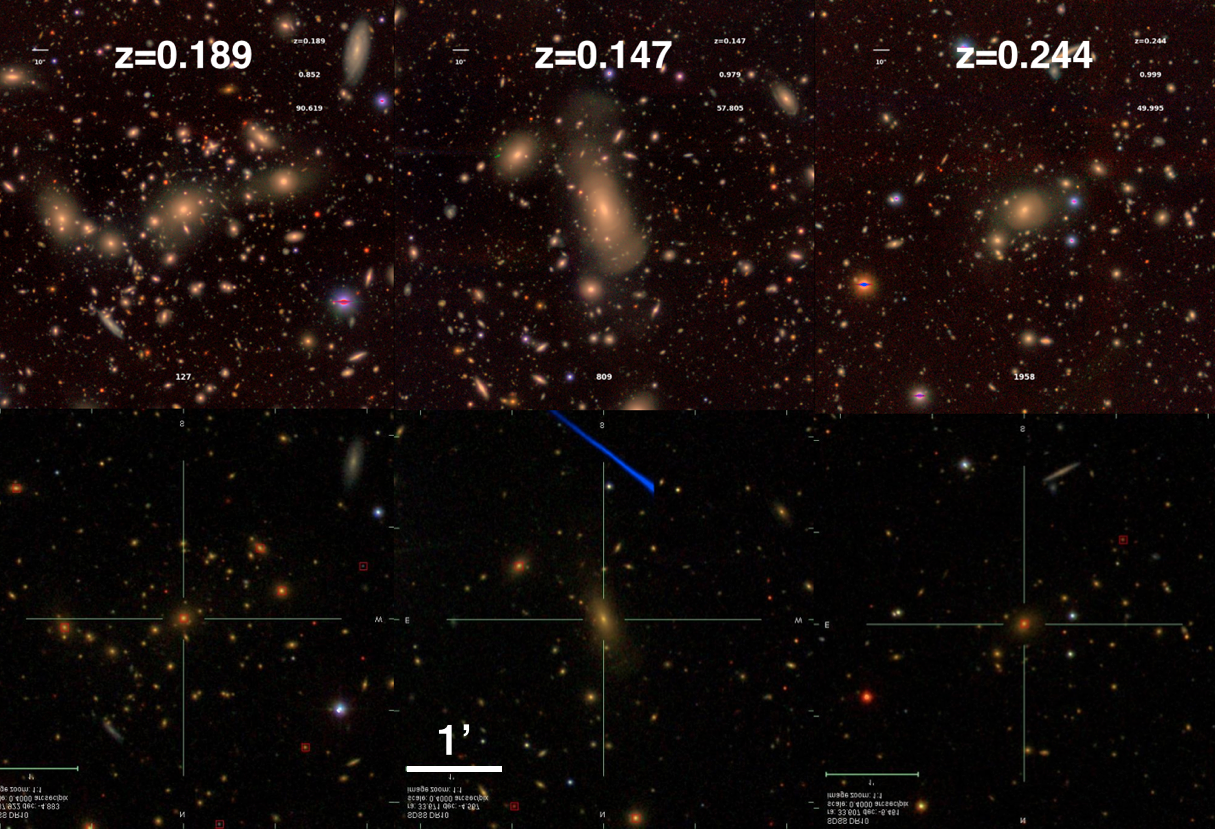
\includegraphics[width=16.5cm]{fig/fig1.png}
    \caption{
   Cartoons that illustrate the basic idea of the proposed method for the
   estimation of average merger mass ratio.  The style is adopted from Faber\etal (2007).
   The upper panels show the basic
   picture of the ``two-phase'' formation scenario. The lower panel describes
   a general picture for the evolution of massive galaxies on the
   $M_{\ast}$-color plane.  After massive ETGs were quenched, they quickly
   moved to the red-sequence, and gradually evolved along it as they are
   becoming redder due to the aging of stellar population, and more massive due
   to the accumulation of extended stellar envelope through many minor (dry)
   mergers.  Since the stellar content of smaller system should have lower
   metallicity, the outer envelope naturally has a bluer color compared to inner
   region.  And, such color difference reflects the average mass ratio of all
   mergers that contribute to the second phase of evolution.  Larger color
   difference means more stellar material came from smaller galaxies, hence
   makes minor merger more important.  
   }
   \label{figure:1}
\end{figure}

%%%%%%%%%%%%: End of the File %%%%%%%%%%%%

\end{CJK*}

\clearpage 

%%%%%%%%%%%: Possible Tables %%%%%%%%%%%%%
%\begin{deluxetable}{c ccc cc cc}[b!]
\tabletypesize{\scriptsize}
\tablewidth{0pt}
\tablecolumns{8}
\tablenum{1}
\tablecaption{Average \mden{} Profiles of Massive Galaxies in Different Stellar Mass Bins}
%% ------------------------------------------------------------------------------------ %% 
\tablehead{
    \colhead{Radius} & 
    \multicolumn{3}{c}{[\mden{}]; Combined samples} &
    \multicolumn{2}{c}{[\mden{}]; $M_{\star,100\ \mathrm{kpc}}$-matched} &
    \multicolumn{2}{c}{[\mden{}]; $M_{\star,10\ \mathrm{kpc}}$-matched}
	\vspace{1.4ex}
    %------------------------------------------------------------------------------------%
    \nl 
    \colhead{kpc} & 
    \multicolumn{3}{c}{$\log (M_{\odot}/\mathrm{kpc}^2)$} &
    \multicolumn{2}{c}{$\log (M_{\odot}/\mathrm{kpc}^2)$} &
    \multicolumn{2}{c}{$\log (M_{\odot}/\mathrm{kpc}^2)$}
	\vspace{1.4ex}
    %------------------------------------------------------------------------------------%
    \nl 
    \colhead{} & 
    \colhead{$\log \frac{M_{\star,100\mathrm{kpc}}}{M_{\odot}}\in$[11.4, 11.6]} & 
    \colhead{[11.6, 11.8]} & 
    \colhead{[11.8, 12.0]}\hspace{2.0ex} & 
    \colhead{\texttt{cenHighMh}} & 
    \colhead{\texttt{cenLowMh}} & 
    \colhead{\texttt{cenHighMh}}\hspace{2.0ex} & 
    \colhead{\texttt{cenLowMh}}
    %------------------------------------------------------------------------------------%
	\vspace{1.6ex}
    %------------------------------------------------------------------------------------%
    \nl
    \colhead{    (1)} &
    \colhead{    (2)} &
    \colhead{    (3)} &
    \colhead{    (4)} &
    \colhead{    (5)} &
    \colhead{    (6)} &
    \colhead{    (7)} &
    \colhead{    (8)}
    %------------------------------------------------------------------------------------%
}
%% ------------------------------------------------------------------------------------ %% 
\startdata
%% ------------------------------------------------------------------------------------ %% 

0.0 & $ 9.23\substack{+0.00 \\ -0.00}$ &$ 9.31\substack{+0.00 \\ -0.01}$ &$ 9.32\substack{+0.01 \\ -0.01}$ &$ 9.31\substack{+0.02 \\ -0.02}$ &$ 9.34\substack{+0.01 \\ -0.01}$ &$ 9.31\substack{+0.02 \\ -0.02}$ &$ 9.34\substack{+0.02 \\ -0.02}$ \\
 0.6 & $ 9.20\substack{+0.00 \\ -0.00}$ &$ 9.28\substack{+0.00 \\ -0.01}$ &$ 9.29\substack{+0.01 \\ -0.01}$ &$ 9.27\substack{+0.02 \\ -0.02}$ &$ 9.31\substack{+0.01 \\ -0.01}$ &$ 9.28\substack{+0.02 \\ -0.02}$ &$ 9.31\substack{+0.02 \\ -0.02}$ \\
 1.0 & $ 9.16\substack{+0.00 \\ -0.00}$ &$ 9.24\substack{+0.00 \\ -0.00}$ &$ 9.26\substack{+0.01 \\ -0.01}$ &$ 9.24\substack{+0.02 \\ -0.02}$ &$ 9.27\substack{+0.01 \\ -0.01}$ &$ 9.25\substack{+0.02 \\ -0.02}$ &$ 9.27\substack{+0.02 \\ -0.02}$ \\
 1.4 & $ 9.12\substack{+0.00 \\ -0.00}$ &$ 9.20\substack{+0.00 \\ -0.00}$ &$ 9.23\substack{+0.01 \\ -0.01}$ &$ 9.20\substack{+0.02 \\ -0.02}$ &$ 9.23\substack{+0.01 \\ -0.01}$ &$ 9.21\substack{+0.02 \\ -0.01}$ &$ 9.23\substack{+0.02 \\ -0.01}$ \\
 1.7 & $ 9.06\substack{+0.00 \\ -0.00}$ &$ 9.15\substack{+0.00 \\ -0.00}$ &$ 9.19\substack{+0.01 \\ -0.01}$ &$ 9.15\substack{+0.02 \\ -0.02}$ &$ 9.19\substack{+0.01 \\ -0.01}$ &$ 9.16\substack{+0.01 \\ -0.01}$ &$ 9.18\substack{+0.01 \\ -0.01}$ \\
 2.0 & $ 9.00\substack{+0.00 \\ -0.00}$ &$ 9.10\substack{+0.00 \\ -0.00}$ &$ 9.15\substack{+0.01 \\ -0.01}$ &$ 9.09\substack{+0.01 \\ -0.02}$ &$ 9.13\substack{+0.01 \\ -0.01}$ &$ 9.11\substack{+0.01 \\ -0.01}$ &$ 9.12\substack{+0.01 \\ -0.01}$ \\
 2.4 & $ 8.93\substack{+0.00 \\ -0.00}$ &$ 9.03\substack{+0.00 \\ -0.00}$ &$ 9.09\substack{+0.01 \\ -0.01}$ &$ 9.03\substack{+0.02 \\ -0.02}$ &$ 9.07\substack{+0.01 \\ -0.01}$ &$ 9.05\substack{+0.01 \\ -0.01}$ &$ 9.05\substack{+0.01 \\ -0.01}$ \\
 2.7 & $ 8.87\substack{+0.00 \\ -0.00}$ &$ 8.97\substack{+0.00 \\ -0.00}$ &$ 9.04\substack{+0.01 \\ -0.01}$ &$ 8.97\substack{+0.01 \\ -0.01}$ &$ 9.01\substack{+0.01 \\ -0.01}$ &$ 9.00\substack{+0.01 \\ -0.01}$ &$ 8.99\substack{+0.01 \\ -0.01}$ \\
 3.0 & $ 8.80\substack{+0.00 \\ -0.00}$ &$ 8.90\substack{+0.00 \\ -0.00}$ &$ 8.98\substack{+0.01 \\ -0.01}$ &$ 8.90\substack{+0.01 \\ -0.01}$ &$ 8.95\substack{+0.01 \\ -0.01}$ &$ 8.93\substack{+0.01 \\ -0.01}$ &$ 8.92\substack{+0.01 \\ -0.01}$ \\
 3.4 & $ 8.72\substack{+0.00 \\ -0.00}$ &$ 8.83\substack{+0.00 \\ -0.00}$ &$ 8.92\substack{+0.01 \\ -0.01}$ &$ 8.83\substack{+0.01 \\ -0.01}$ &$ 8.88\substack{+0.01 \\ -0.01}$ &$ 8.86\substack{+0.01 \\ -0.01}$ &$ 8.85\substack{+0.01 \\ -0.01}$ \\
 3.7 & $ 8.66\substack{+0.00 \\ -0.00}$ &$ 8.78\substack{+0.00 \\ -0.00}$ &$ 8.87\substack{+0.01 \\ -0.01}$ &$ 8.78\substack{+0.01 \\ -0.01}$ &$ 8.83\substack{+0.01 \\ -0.01}$ &$ 8.81\substack{+0.01 \\ -0.01}$ &$ 8.79\substack{+0.01 \\ -0.01}$ \\
 4.1 & $ 8.60\substack{+0.00 \\ -0.00}$ &$ 8.72\substack{+0.00 \\ -0.00}$ &$ 8.82\substack{+0.01 \\ -0.01}$ &$ 8.72\substack{+0.01 \\ -0.01}$ &$ 8.77\substack{+0.01 \\ -0.01}$ &$ 8.76\substack{+0.01 \\ -0.01}$ &$ 8.73\substack{+0.01 \\ -0.01}$ \\
 4.4 & $ 8.54\substack{+0.00 \\ -0.00}$ &$ 8.66\substack{+0.00 \\ -0.00}$ &$ 8.77\substack{+0.01 \\ -0.01}$ &$ 8.66\substack{+0.01 \\ -0.01}$ &$ 8.72\substack{+0.01 \\ -0.01}$ &$ 8.70\substack{+0.01 \\ -0.01}$ &$ 8.67\substack{+0.01 \\ -0.01}$ \\
 4.8 & $ 8.48\substack{+0.00 \\ -0.00}$ &$ 8.60\substack{+0.00 \\ -0.00}$ &$ 8.71\substack{+0.01 \\ -0.01}$ &$ 8.60\substack{+0.01 \\ -0.01}$ &$ 8.66\substack{+0.01 \\ -0.01}$ &$ 8.65\substack{+0.01 \\ -0.01}$ &$ 8.61\substack{+0.01 \\ -0.01}$ \\
 6.2 & $ 8.26\substack{+0.00 \\ -0.00}$ &$ 8.40\substack{+0.00 \\ -0.00}$ &$ 8.53\substack{+0.01 \\ -0.01}$ &$ 8.41\substack{+0.01 \\ -0.01}$ &$ 8.46\substack{+0.01 \\ -0.01}$ &$ 8.46\substack{+0.02 \\ -0.02}$ &$ 8.40\substack{+0.02 \\ -0.02}$ \\
 7.6 & $ 8.09\substack{+0.00 \\ -0.00}$ &$ 8.24\substack{+0.00 \\ -0.00}$ &$ 8.39\substack{+0.01 \\ -0.01}$ &$ 8.27\substack{+0.01 \\ -0.01}$ &$ 8.31\substack{+0.01 \\ -0.01}$ &$ 8.31\substack{+0.02 \\ -0.02}$ &$ 8.23\substack{+0.02 \\ -0.02}$ \\
 9.0 & $ 7.95\substack{+0.00 \\ -0.00}$ &$ 8.10\substack{+0.00 \\ -0.00}$ &$ 8.27\substack{+0.01 \\ -0.01}$ &$ 8.14\substack{+0.02 \\ -0.02}$ &$ 8.18\substack{+0.01 \\ -0.01}$ &$ 8.19\substack{+0.02 \\ -0.02}$ &$ 8.09\substack{+0.02 \\ -0.02}$ \\
10.3 & $ 7.82\substack{+0.00 \\ -0.00}$ &$ 7.99\substack{+0.00 \\ -0.00}$ &$ 8.16\substack{+0.01 \\ -0.01}$ &$ 8.03\substack{+0.02 \\ -0.01}$ &$ 8.06\substack{+0.01 \\ -0.01}$ &$ 8.09\substack{+0.02 \\ -0.02}$ &$ 7.97\substack{+0.02 \\ -0.02}$ \\
11.7 & $ 7.70\substack{+0.00 \\ -0.00}$ &$ 7.88\substack{+0.00 \\ -0.00}$ &$ 8.06\substack{+0.01 \\ -0.01}$ &$ 7.93\substack{+0.02 \\ -0.02}$ &$ 7.96\substack{+0.01 \\ -0.01}$ &$ 7.99\substack{+0.02 \\ -0.02}$ &$ 7.85\substack{+0.02 \\ -0.02}$ \\
13.0 & $ 7.60\substack{+0.00 \\ -0.00}$ &$ 7.78\substack{+0.00 \\ -0.00}$ &$ 7.98\substack{+0.01 \\ -0.01}$ &$ 7.85\substack{+0.02 \\ -0.02}$ &$ 7.87\substack{+0.01 \\ -0.01}$ &$ 7.90\substack{+0.02 \\ -0.02}$ &$ 7.75\substack{+0.02 \\ -0.02}$ \\
14.5 & $ 7.50\substack{+0.00 \\ -0.00}$ &$ 7.69\substack{+0.00 \\ -0.00}$ &$ 7.90\substack{+0.01 \\ -0.01}$ &$ 7.76\substack{+0.02 \\ -0.02}$ &$ 7.78\substack{+0.01 \\ -0.01}$ &$ 7.82\substack{+0.02 \\ -0.02}$ &$ 7.65\substack{+0.02 \\ -0.02}$ \\
16.0 & $ 7.39\substack{+0.00 \\ -0.00}$ &$ 7.60\substack{+0.00 \\ -0.00}$ &$ 7.82\substack{+0.01 \\ -0.01}$ &$ 7.68\substack{+0.02 \\ -0.02}$ &$ 7.69\substack{+0.01 \\ -0.01}$ &$ 7.74\substack{+0.02 \\ -0.03}$ &$ 7.56\substack{+0.02 \\ -0.03}$ \\
17.3 & $ 7.31\substack{+0.00 \\ -0.00}$ &$ 7.52\substack{+0.00 \\ -0.00}$ &$ 7.76\substack{+0.01 \\ -0.01}$ &$ 7.61\substack{+0.02 \\ -0.02}$ &$ 7.62\substack{+0.01 \\ -0.01}$ &$ 7.67\substack{+0.03 \\ -0.03}$ &$ 7.48\substack{+0.03 \\ -0.03}$ \\
18.7 & $ 7.23\substack{+0.00 \\ -0.00}$ &$ 7.45\substack{+0.00 \\ -0.00}$ &$ 7.69\substack{+0.01 \\ -0.01}$ &$ 7.55\substack{+0.02 \\ -0.02}$ &$ 7.55\substack{+0.01 \\ -0.01}$ &$ 7.61\substack{+0.03 \\ -0.03}$ &$ 7.40\substack{+0.03 \\ -0.03}$ \\
22.6 & $ 7.02\substack{+0.00 \\ -0.00}$ &$ 7.27\substack{+0.00 \\ -0.00}$ &$ 7.54\substack{+0.01 \\ -0.01}$ &$ 7.38\substack{+0.02 \\ -0.02}$ &$ 7.37\substack{+0.01 \\ -0.01}$ &$ 7.45\substack{+0.03 \\ -0.03}$ &$ 7.21\substack{+0.03 \\ -0.03}$ \\
26.1 & $ 6.86\substack{+0.00 \\ -0.00}$ &$ 7.12\substack{+0.00 \\ -0.00}$ &$ 7.41\substack{+0.01 \\ -0.01}$ &$ 7.25\substack{+0.02 \\ -0.02}$ &$ 7.24\substack{+0.01 \\ -0.01}$ &$ 7.32\substack{+0.03 \\ -0.03}$ &$ 7.05\substack{+0.03 \\ -0.03}$ \\
30.0 & $ 6.70\substack{+0.00 \\ -0.00}$ &$ 6.98\substack{+0.00 \\ -0.00}$ &$ 7.29\substack{+0.01 \\ -0.01}$ &$ 7.13\substack{+0.03 \\ -0.02}$ &$ 7.10\substack{+0.01 \\ -0.01}$ &$ 7.20\substack{+0.03 \\ -0.04}$ &$ 6.90\substack{+0.03 \\ -0.04}$ \\
33.7 & $ 6.55\substack{+0.00 \\ -0.00}$ &$ 6.85\substack{+0.01 \\ -0.01}$ &$ 7.18\substack{+0.01 \\ -0.01}$ &$ 7.01\substack{+0.03 \\ -0.03}$ &$ 6.98\substack{+0.01 \\ -0.01}$ &$ 7.09\substack{+0.03 \\ -0.03}$ &$ 6.76\substack{+0.03 \\ -0.03}$ \\
37.8 & $ 6.41\substack{+0.00 \\ -0.00}$ &$ 6.72\substack{+0.01 \\ -0.01}$ &$ 7.07\substack{+0.01 \\ -0.01}$ &$ 6.90\substack{+0.03 \\ -0.03}$ &$ 6.85\substack{+0.01 \\ -0.01}$ &$ 6.98\substack{+0.04 \\ -0.04}$ &$ 6.63\substack{+0.04 \\ -0.04}$ \\
41.6 & $ 6.29\substack{+0.01 \\ -0.01}$ &$ 6.61\substack{+0.01 \\ -0.01}$ &$ 6.98\substack{+0.01 \\ -0.01}$ &$ 6.81\substack{+0.03 \\ -0.03}$ &$ 6.75\substack{+0.01 \\ -0.01}$ &$ 6.89\substack{+0.04 \\ -0.04}$ &$ 6.51\substack{+0.04 \\ -0.04}$ \\
45.7 & $ 6.17\substack{+0.01 \\ -0.01}$ &$ 6.50\substack{+0.01 \\ -0.01}$ &$ 6.88\substack{+0.01 \\ -0.01}$ &$ 6.71\substack{+0.03 \\ -0.03}$ &$ 6.64\substack{+0.01 \\ -0.01}$ &$ 6.79\substack{+0.04 \\ -0.04}$ &$ 6.39\substack{+0.04 \\ -0.04}$ \\
49.3 & $ 6.07\substack{+0.01 \\ -0.01}$ &$ 6.41\substack{+0.01 \\ -0.01}$ &$ 6.80\substack{+0.01 \\ -0.02}$ &$ 6.62\substack{+0.03 \\ -0.03}$ &$ 6.56\substack{+0.01 \\ -0.01}$ &$ 6.70\substack{+0.04 \\ -0.04}$ &$ 6.30\substack{+0.04 \\ -0.04}$ \\
53.1 & $ 5.98\substack{+0.01 \\ -0.01}$ &$ 6.33\substack{+0.01 \\ -0.01}$ &$ 6.71\substack{+0.02 \\ -0.02}$ &$ 6.55\substack{+0.03 \\ -0.03}$ &$ 6.46\substack{+0.01 \\ -0.01}$ &$ 6.64\substack{+0.04 \\ -0.04}$ &$ 6.21\substack{+0.04 \\ -0.04}$ \\
57.2 & $ 5.88\substack{+0.01 \\ -0.01}$ &$ 6.24\substack{+0.01 \\ -0.01}$ &$ 6.63\substack{+0.02 \\ -0.02}$ &$ 6.47\substack{+0.04 \\ -0.04}$ &$ 6.37\substack{+0.01 \\ -0.01}$ &$ 6.56\substack{+0.04 \\ -0.04}$ &$ 6.11\substack{+0.04 \\ -0.04}$ \\
61.5 & $ 5.79\substack{+0.01 \\ -0.01}$ &$ 6.15\substack{+0.01 \\ -0.01}$ &$ 6.55\substack{+0.02 \\ -0.02}$ &$ 6.39\substack{+0.04 \\ -0.04}$ &$ 6.29\substack{+0.01 \\ -0.01}$ &$ 6.49\substack{+0.04 \\ -0.04}$ &$ 6.03\substack{+0.04 \\ -0.04}$ \\
66.0 & $ 5.70\substack{+0.01 \\ -0.01}$ &$ 6.05\substack{+0.01 \\ -0.01}$ &$ 6.47\substack{+0.02 \\ -0.02}$ &$ 6.32\substack{+0.04 \\ -0.04}$ &$ 6.20\substack{+0.01 \\ -0.01}$ &$ 6.37\substack{+0.05 \\ -0.06}$ &$ 5.94\substack{+0.05 \\ -0.06}$ \\
69.8 & $ 5.64\substack{+0.01 \\ -0.01}$ &$ 5.98\substack{+0.01 \\ -0.01}$ &$ 6.40\substack{+0.02 \\ -0.02}$ &$ 6.25\substack{+0.04 \\ -0.04}$ &$ 6.12\substack{+0.02 \\ -0.01}$ &$ 6.35\substack{+0.04 \\ -0.05}$ &$ 5.87\substack{+0.04 \\ -0.05}$ \\
74.7 & $ 5.56\substack{+0.01 \\ -0.01}$ &$ 5.89\substack{+0.01 \\ -0.01}$ &$ 6.32\substack{+0.02 \\ -0.02}$ &$ 6.18\substack{+0.04 \\ -0.04}$ &$ 6.04\substack{+0.02 \\ -0.02}$ &$ 6.28\substack{+0.05 \\ -0.05}$ &$ 5.79\substack{+0.05 \\ -0.05}$ \\
79.9 & $ 5.49\substack{+0.01 \\ -0.01}$ &$ 5.81\substack{+0.01 \\ -0.01}$ &$ 6.24\substack{+0.02 \\ -0.02}$ &$ 6.12\substack{+0.04 \\ -0.04}$ &$ 5.96\substack{+0.02 \\ -0.02}$ &$ 6.20\substack{+0.05 \\ -0.06}$ &$ 5.72\substack{+0.05 \\ -0.06}$ \\
84.3 & $ 5.43\substack{+0.01 \\ -0.01}$ &$ 5.74\substack{+0.01 \\ -0.01}$ &$ 6.18\substack{+0.02 \\ -0.02}$ &$ 6.05\substack{+0.04 \\ -0.05}$ &$ 5.89\substack{+0.02 \\ -0.02}$ &$ 6.16\substack{+0.05 \\ -0.05}$ &$ 5.65\substack{+0.05 \\ -0.05}$ \\
88.8 & $ 5.38\substack{+0.01 \\ -0.01}$ &$ 5.67\substack{+0.01 \\ -0.01}$ &$ 6.11\substack{+0.02 \\ -0.02}$ &$ 5.99\substack{+0.05 \\ -0.06}$ &$ 5.81\substack{+0.02 \\ -0.02}$ &$ 6.08\substack{+0.05 \\ -0.06}$ &$ 5.58\substack{+0.05 \\ -0.06}$ \\
97.2 & $ 5.29\substack{+0.01 \\ -0.01}$ &$ 5.56\substack{+0.01 \\ -0.01}$ &$ 5.98\substack{+0.02 \\ -0.02}$ &$ 5.92\substack{+0.04 \\ -0.04}$ &$ 5.69\substack{+0.02 \\ -0.02}$ &$ 5.99\substack{+0.05 \\ -0.05}$ &$ 5.47\substack{+0.05 \\ -0.05}$ \\
103.6 & $ 5.21\substack{+0.01 \\ -0.01}$ &$ 5.49\substack{+0.01 \\ -0.01}$ &$ 5.89\substack{+0.03 \\ -0.03}$ &$ 5.84\substack{+0.05 \\ -0.05}$ &$ 5.62\substack{+0.02 \\ -0.02}$ &$ 5.94\substack{+0.05 \\ -0.05}$ &$ 5.39\substack{+0.05 \\ -0.05}$ \\
111.6 & $ 5.14\substack{+0.01 \\ -0.01}$ &$ 5.40\substack{+0.01 \\ -0.01}$ &$ 5.79\substack{+0.03 \\ -0.03}$ &$ 5.78\substack{+0.05 \\ -0.05}$ &$ 5.54\substack{+0.02 \\ -0.02}$ &$ 5.87\substack{+0.05 \\ -0.05}$ &$ 5.32\substack{+0.05 \\ -0.05}$ \\
117.2 & $ 5.10\substack{+0.01 \\ -0.01}$ &$ 5.36\substack{+0.01 \\ -0.01}$ &$ 5.72\substack{+0.03 \\ -0.03}$ &$ 5.72\substack{+0.05 \\ -0.05}$ &$ 5.47\substack{+0.02 \\ -0.02}$ &$ 5.82\substack{+0.05 \\ -0.05}$ &$ 5.29\substack{+0.05 \\ -0.05}$ \\
129.0 & $ 5.00\substack{+0.01 \\ -0.01}$ &$ 5.25\substack{+0.02 \\ -0.02}$ &$ 5.61\substack{+0.03 \\ -0.03}$ &$ 5.64\substack{+0.05 \\ -0.05}$ &$ 5.36\substack{+0.02 \\ -0.02}$ &$ 5.74\substack{+0.05 \\ -0.05}$ &$ 5.21\substack{+0.05 \\ -0.05}$ \\
141.7 & $ 4.89\substack{+0.02 \\ -0.02}$ &$ 5.13\substack{+0.02 \\ -0.02}$ &$ 5.49\substack{+0.03 \\ -0.03}$ &$ 5.58\substack{+0.05 \\ -0.05}$ &$ 5.23\substack{+0.03 \\ -0.03}$ &$ 5.66\substack{+0.05 \\ -0.05}$ &$ 5.09\substack{+0.05 \\ -0.05}$ \\
146.7 & $ 4.85\substack{+0.02 \\ -0.02}$ &$ 5.10\substack{+0.02 \\ -0.02}$ &$ 5.46\substack{+0.03 \\ -0.03}$ &$ 5.51\substack{+0.06 \\ -0.06}$ &$ 5.19\substack{+0.03 \\ -0.03}$ &$ 5.61\substack{+0.05 \\ -0.05}$ &$ 5.03\substack{+0.05 \\ -0.05}$ \\

%%------------------------------------------------------------------------------------ %% 
\enddata
%% ------------------------------------------------------------------------------------ %% 
\tablecomments{
    Average \mden{} profiles of massive \rbcg{} and \nbcg{} galaxies in different
    samples:\\ 
    Col.~(1) Radius along the major axis in kpc.\\
    Col.~(2) Average \mden{} profile for galaxies with 
        $11.4 \leq$\logmtot$< 11.6$ in the combined samples of \rbcg{} and \nbcg{}
        galaxies. \\ 
    Col.~(3) Average \mden{} profile of combined samples in the mass bin of 
        $11.6 \leq$\logmtot$< 11.8$. \\ 
    Col.~(4) Average \mden{} profile of combined samples in the mass bin of 
        $11.8 \leq$\logmtot$< 12.0$. \\ 
    Col.~(5) and Col.~(6) are the average \mden{} profiles of \rbcg{} and \nbcg{} galaxies
        in the \mtot{}-matched samples within $11.6 \leq$\logmtot{}$< 11.9$. \\ 
    Col.~(7) and Col.~(8) are the average \mden{} profiles of \rbcg{} and \nbcg{} galaxies 
        in the \minn{}-matched samples within $11.2 \leq$\logmtot{}$< 11.6$. \\ 
    The upper and lower uncertainties of these average profiles vial bootstrap-resampling 
    method are also displayed.
}
\label{tab:prof}
\end{deluxetable}


\end{document}
